\chapter{Аналитический раздел}

В этом разделе будет рассмотрен шифровальный алгоритм AES в режиме шифрования CFB.

\section{Алгоритм AES}

Шифровальная алгоритм AES (англ. \textit{Advanced Encryption Standart} --- AES) --- симметричный блочнный шифровальный алгоритм, разработанный в 2001 году Национальный институтом стандартов и технологий США. Он использует блочное шифрование, длина блока фиксирована и равна 128 битам, длина ключа 128, 192 либо же 256 бит. Он состоит раундов шифрования,количество которых зависит от длины ключа: 10 раундов для ключа размером 128 бит, 12 раундов для ключа размером 192 бита и 14 раундов для ключа размером 256 бит.

Прежде чем перейти к раундам шифрования, происходит генерация ключей раунда (раундовых ключей) из исходного ключа, Рассмотрим, как это происходит.

\subsection{Получение ключей раунда}

Определим фунцию $g$, изменяющую четырёхбайтовое слово так, как указано на рисунке \ref{img:g_function}.

Ключей раундов $k_{i}$ необходимо на 1 больше, чем количество раундов, т.е. 11 ключей раундов для основногоключа длиной 128 бит, 13 ключей раунда для основного ключа длиной 192 бита и 15 ключей раунда для основного ключа длинной 256 бит.

\clearpage

\includeimage
{g_function} % Имя файла без расширения (файл должен быть расположен в директории inc/img/)
{f} % Обтекание (без обтекания)
{ht!} % Положение рисунка (см. figure из пакета float)
{0.6\textwidth} % Ширина рисунка
{Схема функции g} % Подпись рисунка

%\begin{figure}[ht!]
%	\centering
%	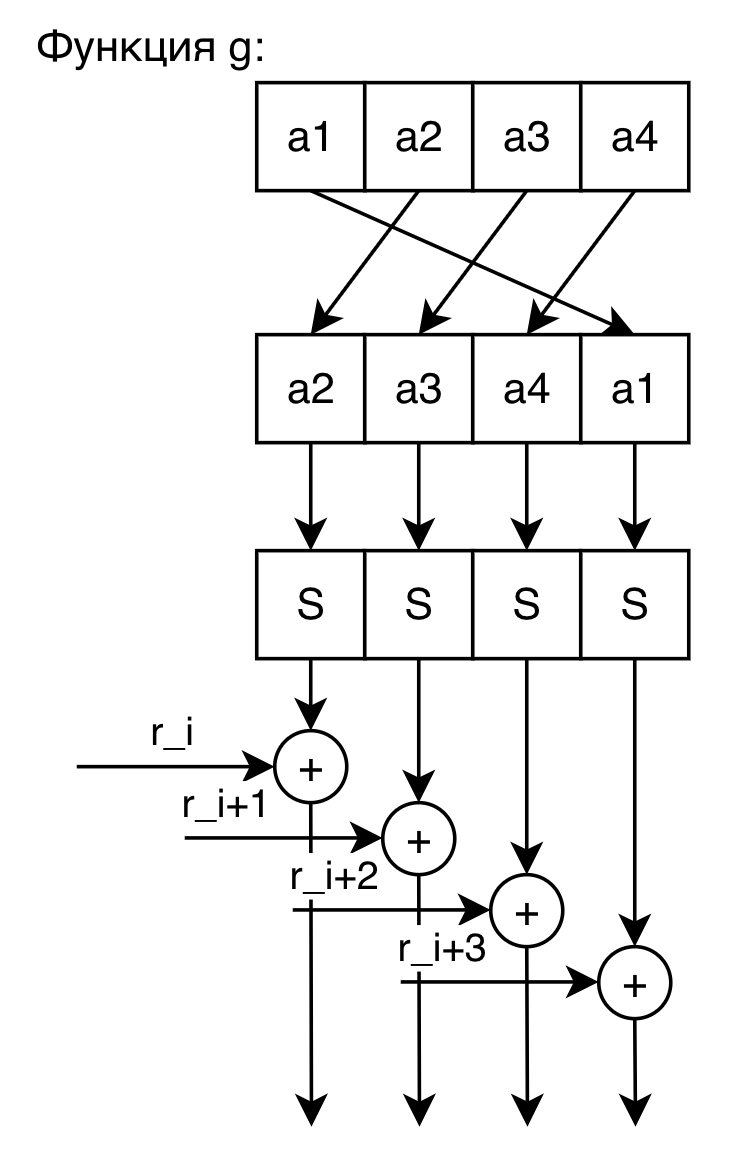
\includegraphics[width=0.6\linewidth]{img/g_function.png}
%	\caption{Схема функции g}
%	\label{img:g_function}
%\end{figure}

\clearpage

Алгоритм получения ключа раунда из исходного ключа преставлен в виде схемы алгоритма на рисунке \ref{img:round_keys}.

\includeimage
{round_keys} % Имя файла без расширения (файл должен быть расположен в директории inc/img/)
{f} % Обтекание (без обтекания)
{ht!} % Положение рисунка (см. figure из пакета float)
{0.6\textwidth} % Ширина рисунка
{Схема алгоритма получения ключей раунда} % Подпись рисунка

%\begin{figure}[ht!]
%	\centering
%	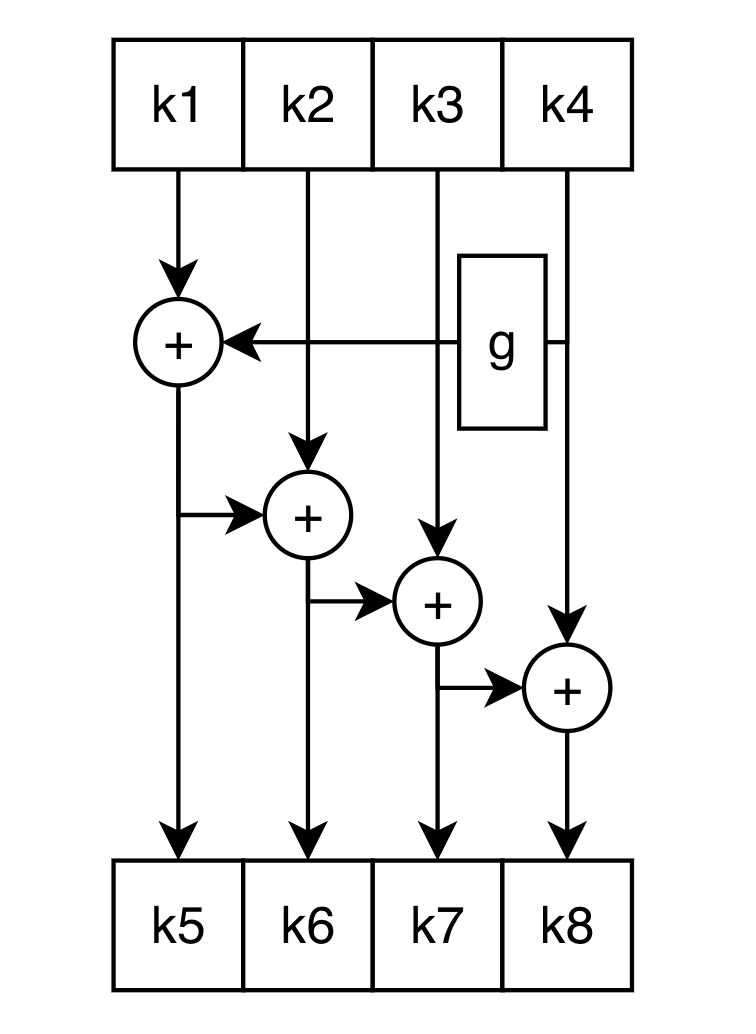
\includegraphics[width=0.6\linewidth]{img/round_keys.png}
%	\caption{Схема функции g}
%	\label{img:round_keys}
%\end{figure}

\subsection{Раунд шифрования}

Раунд шифрования состоит из 5 следующих этапов
\begin{enumerate}[label=\arabic*)]
	\item замена (англ. \textit{confussion});
	\item процедура перестановки строк (англ. \textit{row-row mix procedure} --- RR);
	\item процедура перестановки столбцов (англ. \textit{row-columns mix} --- RC);
	\item смешивание ключа (англ. \textit{key mixing} --- KM).
\end{enumerate}

Замена обеспечивает нелинейность алгоритма шифрования, обрабатываая каждый байт состояния, производя нелинейную замену байт с использованием таблицы замен.

Процедура перестановки строк представляет из себя циклический сдвиг строки состояний на количество байт, зависящее от номера строки.

Процедура перестановки столбцов 4 байта каждого столбца смешиваются с использовоанием обратимой линейной трансформации. На последнем раунду эта процедура не выполняется.

Смешивание ключа представляет из себя операцию XOR с ключом раунда, полученным заранее.

\section{Режимы работы алгоритма AES}

Режим шифрования --- метод применения блочного шифра, позволяющий преобразовать последовательность блоков открытых данных в последовательность блоков зашифрованных данных.

Для AES рекомендованы следующие режими работы:
\begin{enumerate}[label=\arabic*)]
	\item режим электронной кодовой книги (англ. \textit{Electronic Code Bloc} --- ECB);
	\item режим сцепления блоков (англ. \textit{Cipher Block Chaining} -- CBC);
	\item режим параллельноого сцепления блоков (англ. \textit{Parallel Cipher Block Chaining} -- PCBC);
	\item режим обратной связи по шифротексту (англ. \textit{Cipher Feed Back} --- CFB);
	\item режим обратной связи по выходу (англ. \textit{Output Feed Back} --- OFB).
\end{enumerate}

\section{Режимы работы алгоритма CFB}

Алгоритм CFB схематично представлен на рисунке \ref{img:cfb}.
Суть алгоритма заключается в том, что изначально берется блок из 128 битов $C_0$, который называется синхропосылкой. 
Вектор инициализации (или результаты прошлого XOR) шифруется алгоритмом AES или DES (в нашем случае AES). 
Затем результат суммируется по модулю 2 с блоком \(C_0\) и при этом результат используется для шифрования следующего блока.
Таким образом каждый блок суммируется с результатом шифрования предыдущего блока.

Особенностью данного режима является распространение ошибки на всесь последующий текст.
Применяется как правило для шифрования потков информации видео и аудио.

\includeimage
{cfb} % Имя файла без расширения (файл должен быть расположен в директории inc/img/)
{f} % Обтекание (без обтекания)
{ht!} % Положение рисунка (см. figure из пакета float)
{0.9\textwidth} % Ширина рисунка
{Обобщенная схема алгоритма режима шифрования СFB} % Подпись рисунка

%\begin{figure}[ht!]
%	\centering
%	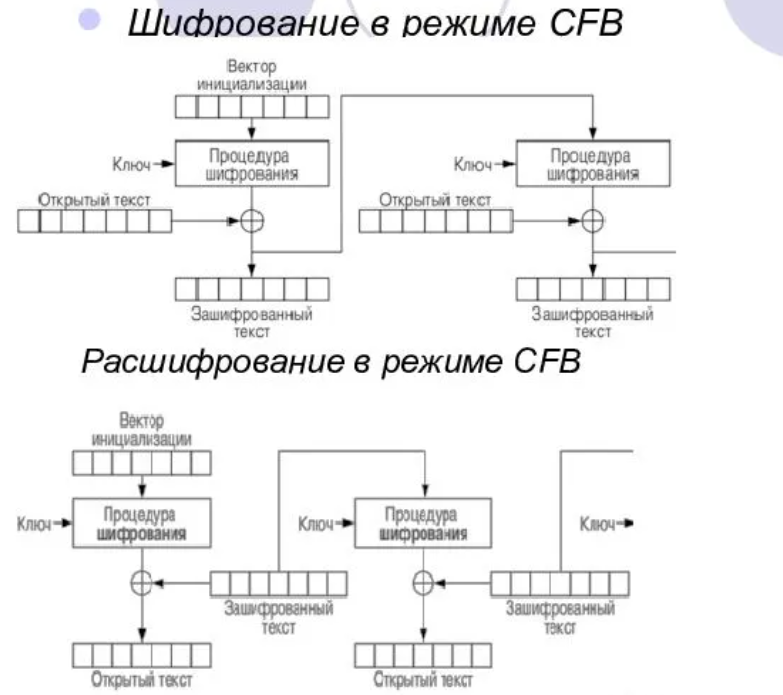
\includegraphics[width=0.9\linewidth]{img/cfb.png}
%	\caption{Обобщенная схема алгоритма режима шифрования СFB}
%	\label{fig:cfb}
%\end{figure}

%\includeimage
%{PCBC} % Имя файла без расширения (файл должен быть расположен в директории inc/img/)
%{f} % Обтекание (без обтекания)
%{H} % Положение рисунка (см. figure из пакета float)
%{0.8\textwidth} % Ширина рисунка
%{Схема режима шифрования PCBC} % Подпись рисунка

\section*{Вывод}

В этом разделе был рассмотрен шифровальный алгоритм AES в режиме шифрования CFB.